\chapter{Introducción general}

En este capítulo se presentan las motivaciones que guiaron la elaboración de este trabajo. Luego se realiza una revisión del estado del arte en cuanto a los productos comerciales disponibles, se describe la propuesta inicial y las razones por las que posteriormente se decidió descartarla, y se exponen el alcance y los objetivos de la propuesta final.

\label{cap:IntroGeneral}

\section{Motivación}

La empresa Trenes Argentinos \cite{web:sofse} adquirió en 2013 un total de 705 unidades eléctricas múltiples (EMU) a la empresa china CRRC Qingdao Sifang \cite{web:sifang} \cite{licitacion1}. Estos vehículos prestan servicios en las líneas Mitre, Sarmiento y Roca desde 2014 \cite{emu:roca} \cite{emu:mitre-sarmiento}.

\begin{figure}[htbp]
	\centering
	\includegraphics[width=.6\textwidth]{./Figures/1082px-Línea_Mitre_Retiro.jpg}
	\caption[Unidad eléctrica múltiple (EMU)]{Una unidad eléctrica múltiple (EMU) en la estación Retiro de la línea Mitre, en Buenos Aires.\footnotemark}
	\label{fig:emu}
\end{figure}
\footnotetext{Fotografía por Casa Rosada (Argentina Presidencia de la Nación), CC BY-SA 2.0, \url{https://commons.wikimedia.org/w/index.php?curid=39117175}}

Los distintos subsistemas electrónicos presentes en una EMU (control de frenos, control de tracción, control de puertas, paneles de información al pasajero, etc.) están interconectados formando una red de datos. Mediante esta red, los componentes comparten datos de diagnóstico y reciben órdenes de control a distancia. La red interna que se utiliza en las EMU es una implementación del estándar TCN (Train Communication Network, IEC 61375-1 \cite{iec61375-1}). La red TCN es una combinación jerárquica de dos buses de datos: WTB (Wire Train Bus) para interconectar los diferentes vehículos en una formación, y MVB (Multifunction Vehicle Bus) para interconectar los dispositivos dentro de cada vehículo.

Actualmente Trenes Argentinos carece del conocimiento y las herramientas necesarias para interactuar con la red TCN en las EMU, de forma tal de que puedan capturar la información disponible, o agregar dispositivos de desarrollo propio.
Las EMU ofrecen una visualización del estado de algunos componentes en la cabina del conductor, pero no todos los valores están representados.
Tampoco se dispone de un sistema de monitoreo que permita observar dichos valores a distancia.
Se cuenta con un sistema de almacenamiento histórico del estado de los componentes, pero se trata de un sistema propietario que registra solo un subconjunto de los datos disponibles, y por una duración limitada.

Estas limitaciones adquieren relevancia en situaciones frecuentes.
Por ejemplo, cuando una formación queda varada en un punto alejado de una estación, los técnicos se ven obligados a trasladarse personalmente para evaluar el problema, provocando demoras en el servicio.
También es habitual la quema de fusibles, un inconveniente difícil de diagnosticar sin el monitoreo de variables como la tensión de línea.
Otro desafío adicional es la falta de almacenamiento de las variables relacionadas con la temperatura de los coches y el estado del sistema de aire acondicionado, lo que dificulta realizar un análisis del sistema de climatización de forma sencilla.

Con el objetivo de buscar una solución a los problemas mencionados, Trenes Argentinos trabaja en conjunto con el Grupo de Investigación en Calidad y Seguridad de las Aplicaciones Ferroviarias (GICSAFe) \cite{web:gicsafe}. Esta organización desarrolla sistemas electrónicos e informáticos para uso en el ámbito ferroviario, que permiten sustituir importaciones, evitar la dependencia de tecnología cerrada que debe ser mantenida durante décadas, y generar trabajo con alto valor agregado.

\section{Estado del arte}

\label{estadodelarte}

La norma IEC 61375-1 es la fuente de información principal a tener en cuenta respecto del estándar TCN. Lamentablemente, no hay mucha información de libre acceso acerca del estándar, como artículos y notas de aplicación. Entre las publicaciones encontradas que citan a la norma las más relevantes son \textit{Design and implementation of MVB protocol analyzer} \cite{mvb-pub-1} (escrita en idioma chino) y \textit{An MVB signal capturer based on microcontrollers for metro train on-line health monitoring system} \cite{mvb-pub-2}, aunque ambas son demasiado cortas como para aportar información realmente útil.
Otra publicación de interés es \textit{A Novel SoC Architecture for a MVB Slave Node} \cite{mvb-pub-3}, donde se describe el diseño de una arquitectura SoC compatible con el estándar TCN, basado en una FPGA.

La mayoría de los equipos desarrollados hasta la fecha que funcionan de acuerdo al estándar TCN se basan en dos ASICs diferentes: el circuito MVBCS1 \cite{mvbcs1}, producido originalmente por la compañía ABB (aunque hoy en día es comercializado por Siemens) y el MVBC02C \cite{mvbc02c}, producido por Bombardier. Debido a su naturaleza, estos circuitos integrados no son lo suficientemente versátiles como para satisfacer la amplia gama de posibilidades con respecto al tipo de nodos conectados a la red TCN \cite{mvb-pub-3}.

Es posible encontrar en el mercado soluciones integrales, que podrían resolver parcialmente los problemas que afronta Trenes Argentinos. A continuación se presentan algunos de estos dispositivos, así como sus características principales.

\subsection{Yacer -- MVB-Analyzer}

El analizador de protocolo \textit{MVB-Analyzer} de la empresa Yacer \cite{yacer} (fig. \ref{fig:yacer}) proporciona una interfaz MVB, dos interfaces Ethernet y dos interfaces de expansión para recopilar y recibir tramas MVB y WTB, entre otras, y enviarlas a una computadora a través de una interfaz Ethernet. El producto incluye un software que permite analizar los datos del bus MVB y realizar simulaciones para encontrar la resolución de problemas y evaluar el funcionamiento del bus MVB.

\subsection{AMiT Transportation -- WTB and MVB Analyzers}

Los analizadores del bus WTB y MVB de la empresa AMiT Transportation \cite{amit} (fig. \ref{fig:amit}) son dispositivos de bus pasivos que monitorean el tráfico en la red y lo pasan al bus Ethernet en tramas UDP.

El analizador solo monitorea el bus, y es ``invisible'' para otros dispositivos. Se monitorean todas las tramas WTB o MVB en el bus, que son transmitidas por el bus Ethernet. El producto incluye un complemento para el software de código abierto Wireshark \cite{wireshark}, que permite analizar las tramas capturadas con una PC.

\subsection{Duagon -- D442 MVB Diagnostic System}

El sistema de diagnóstico MVB de la empresa Duagon \cite{duagon} (fig. \ref{fig:duagon}) está diseñado para depurar dispositivos y redes MVB. El sistema se conecta a una PC común, y puede funcionar en dos modos de operación:

\begin{itemize}
\item En el modo ``monitor'', el sistema permite investigar dispositivos MVB en el bus, leer y escribir la base de datos MVB, y escanear los puertos de los dispositivos, entre otras cosas.
\item En el modo ``servidor'', el sistema permite ejecutar aplicaciones programadas por el usuario. Se incluye una biblioteca de programación MVB con todas las funciones en el sistema de diagnóstico para controlar una red MVB completa.
\end{itemize}

\begin{figure}[htbp]
	\centering
    \begin{subfigure}[b]{0.45\textwidth}
        \centering
        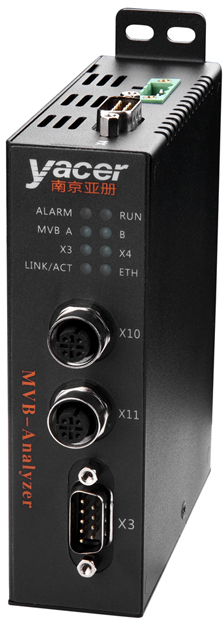
\includegraphics[height=17\baselineskip]{./Figures/yacer.jpg}
        \caption[Yacer -- MVB-Analyzer]{El analizador de protocolo \textit{MVB-Analyzer} de la empresa Yacer.}
        \label{fig:yacer}
    \end{subfigure}
    \hfill
    \begin{subfigure}[b]{0.45\textwidth}
        \centering
        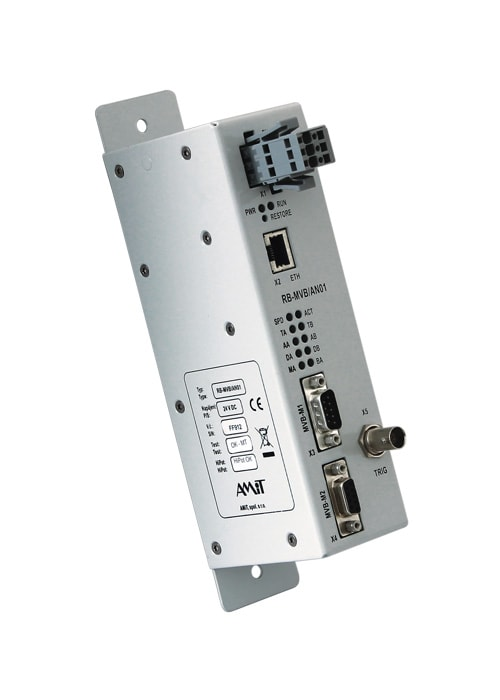
\includegraphics[height=17\baselineskip]{./Figures/amit.jpg}
        \caption[AMiT Transportation -- WTB and MVB Analyzers]{El analizador de bus MVB de la empresa AMiT Transportation.}
        \label{fig:amit}
    \end{subfigure}
    \hfill
    \begin{subfigure}[b]{0.6\textwidth}
        \centering
        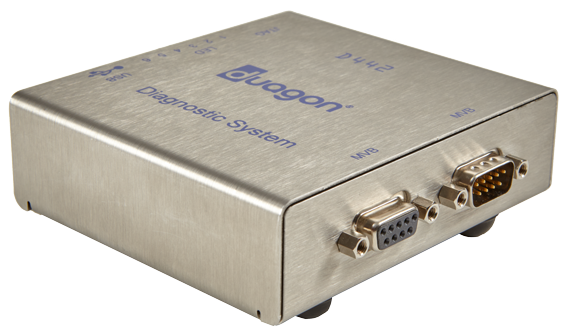
\includegraphics[width=1\textwidth]{./Figures/duagon.png}
        \caption[Duagon -- D442 MVB Diagnostic System]{El sistema de diagnóstico MVB de la empresa Duagon.}
        \label{fig:duagon}
    \end{subfigure}
    \caption{Algunos de los dispositivos de captura disponibles en el mercado.}
\end{figure}

\section{Propuesta inicial}

Si bien los productos listados en la sección \ref{estadodelarte} podrían ser de utilidad para Trenes Argentinos, no resolverían los problemas principales, que son la falta de \emph{know-how} y la dependencia de tecnología cerrada. Por esta razón, el GICSAFe forma varios grupos de trabajo para generar tecnología y conocimiento propio sobre la red TCN. Como parte de esta iniciativa se presenta el Proyecto de Desarrollo Estratégico UBA-PDE Nº 15/2020 \cite{pde2020}, titulado ``Sistema de monitoreo y gestión de la red TCN en formaciones ferroviarias''.

Los objetivos planteados en el PDE son:

\begin{enumerate}
\item Desarrollar un prototipo que permita monitorear la red TCN presente en las formaciones ferroviarias.
\item Que los datos relevados puedan ser reportados a una base de datos remota para poder ser procesados y consultados por Trenes Argentinos en tiempo real.
\item Desarrollar la capacidad de inyectar datos en la red a partir del conocimiento adquirido en las etapas previas.
\end{enumerate}

Para resolver dichos objetivos, se evaluó realizar un prototipo basado en el chip MVBC02C.
Luego de analizar la información disponible acerca del chip, y tras diversas reuniones con autoridades y técnicos de Trenes Argentinos, se decidió abandonar el objetivo de inyectar datos en la red.
Entre las razones se destacan la escasa información disponible acerca del chip MVBC02C, y el riesgo asociado a la seguridad funcional de la formación, ya que por la red TCN circula información crítica, como los sistemas de frenado, tracción y puertas.
Por otro lado, el resultado que podría obtenerse no resulta tan relevante para Trenes Argentinos frente al desafío que esto representa.
Como resultado, se decidió desarrollar un prototipo más simple utilizando un microcontrolador en lugar del chip MVBC02C.

\section{Alcance y objetivos}

En este trabajo se propone realizar un dispositivo que permita monitorear el tráfico de la red TCN, en particular del bus MVB. Los requerimientos principales son:

\begin{enumerate}
\item El dispositivo debe poder conectarse al bus MVB mediante alguno de los conectores disponibles en la formación ferroviaria, de tipo DB9.
\item El dispositivo debe poder capturar y decodificar tramas de la red MVB en tiempo real.
\item El dispositivo debe poder almacenar la información capturada por un tiempo determinado.
\end{enumerate}
